\documentclass[a4paper]{article}

\usepackage[utf8]{inputenc}
\usepackage{graphicx}
\usepackage[export]{adjustbox}
\usepackage{subcaption}
\usepackage{hyperref}
\usepackage{float}

\title{GRACeFUL Visual Editor}
%\author{}
\date{\today}

\begin{document}

\maketitle

The Graceful Visual Editor is a web-based application that supports the policy-making process in Global Systems Science (GSS), specifically in Climate Resilient Urban Design (CRUD).
The current prototype supports the stakeholder participation in visualizing different phases of a policy-making process by providing an interactive graphical interface in which the user can build a system model from building blocks provided by the library (written in the GRACe DSL). This document provides a brief introduction to the editor in Section \ref{intro} and its usability in Section \ref{usability} and its implementation details in Section \ref{implementation}. Please refer to deliverable D2.5 "CRUD RAT Prototype" for complementary information from the design point of view.

\section{Introduction}
\label{intro}
The main elements of the visual editor are the Navigation tab, Tool bar, Graph area, and the Control tab as shown in Figure \ref{fig:layout}. The current prototype provides a widget-based implementation, where each option in the navigation tab represents a step in the policy-making process. The editor loads the tool bar, graph area, and control tab, based on the selected option in the navigation tab. The tool bar on the left provides the building blocks or elements from the library that is obtained from the server. It can be toggled to show and/or hide. The graph area at the center is the canvas area, where the user can draw nodes and links. Please note that the current implementation does not differentiate between a parking lot and the main graph area canvas as proposed in D3.2. i.e., There is a single canvas in the graph area as opposed to two in the initial design and the user would construct the model in this canvas. Finally, the Controls tab consists of a list of controls to assist in building the system model and to interact with the server.

Some of the basic functionalities available in the editor are:
\begin{enumerate}
	\item Create Nodes and Links - A node is created by double-clicking in the graph area. The label of the node is set either by double-clicking on the node or entering it in the label field under the controls tab, after selecting the node. To create a link between nodes, click on the source node to get a dragger object and drag it to the target node as shown in the Figure \ref{fig:node_link}.
		
	\item Delete Nodes and Links - The node can be deleted by either hovering over the node and clicking on the delete icon or selecting the node and clicking on the delete icon in the controls tab as shown in the Figure \ref{fig:delete}. To delete a link, click on the delete icon after selecting the link. The white bubble on the link allows to bend them into curves.
	
	\item Load/Save/Clear - The editor provides the option to save an instance of a model and reuse it later by loading it into the editor. A model could also be cleared completely from the editor.

	\item For every node/link, the editor provides the option to take notes by selecting the node/link and entering the content in the comments field in the control tab. 
	
	\item The visual editor allows zooming in and out, as well as panning of the diagram. The nodes and links can be dragged around in the graph area. 
	
\end{enumerate} 

\begin{figure}[H]
\begin{center}
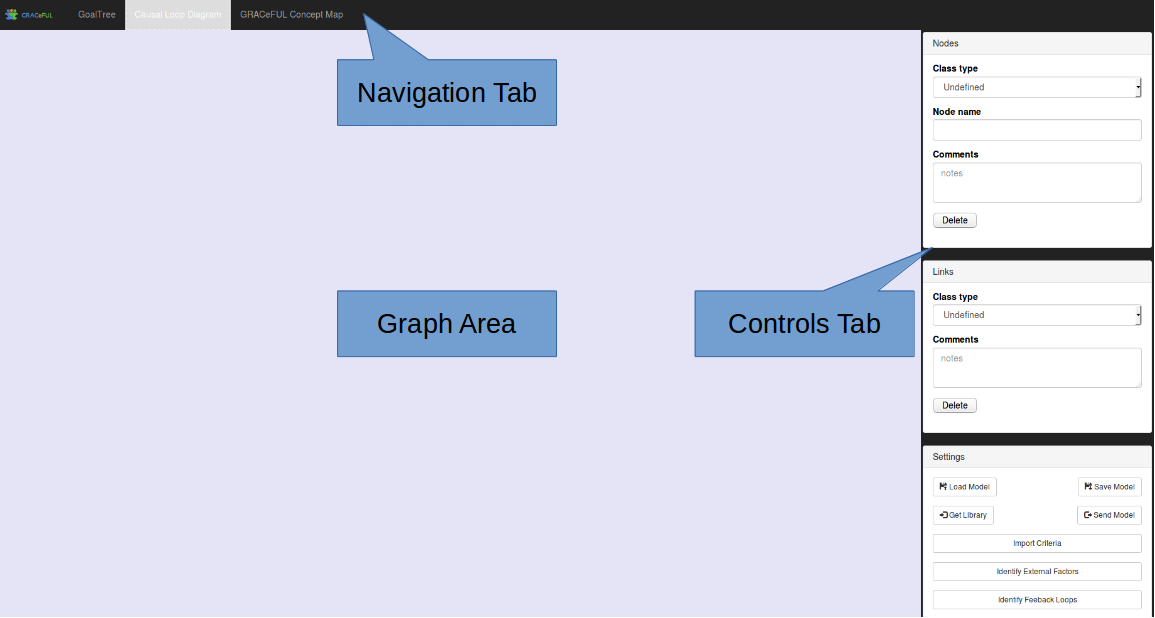
\includegraphics[height=3in,width=5in]{img/layout.png}
\caption{\small \sl Visual Editor Interface.\label{fig:layout}}
\end{center}
\end{figure}

\begin{figure}[H]
 
\begin{subfigure}{0.5\textwidth}
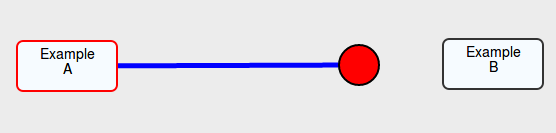
\includegraphics[width=0.8\linewidth, height=2cm]{img/node_link.png} 
\caption{Creation}
\label{fig:node_link}
\end{subfigure}
\begin{subfigure}{0.5\textwidth}
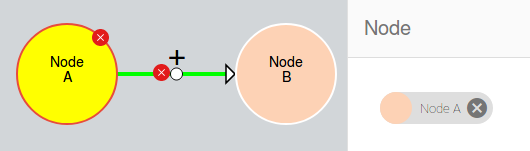
\includegraphics[width=1.2\linewidth, height=2cm]{img/delete_nodeLink.png}
\caption{Deletion}
\label{fig:delete}
\end{subfigure}
 
\caption{Nodes and Links.}
%\label{fig:image2}
\end{figure}

\section{Tool access}
\label{proto}

The current prototype of the GRACeFUL visual editor could be accessed under the link: 

\begin{center}
 \url{http://vocol.iais.fraunhofer.de/graceful-rat/static/index.html}
 \end{center} 

The full source code of this prototype is available in the GitHub repository: 

\begin{center}
\url{https://github.com/GRACeFUL-project/GRACeFULEditor/}
\end{center}

A modern web browser such as Google Chrome or Mozilla Firefox could be used to load the editor. 

\section{Usability}
\label{usability}

The GRACeFUL Concept Map (GCM) modeling is a step-by-step process, which involves Goal Tree, Causal Loop Diagram (CLD), Stakeholder preferences, and Stock Flow Diagram (SFD-like), as described in the deliverable D2.2, section 3.2. Currently these steps are available as separate tabs in the visual editor, but they are all interlinked via a single global model. To build a system model, the modeler would need the GRACeFUL components, which is referred to as \textit{library elements} in the rest of the document. The editor is connected to a backend solver called GRACE (domain specific language for GCM) to fetch the library elements. More technical information of this connection can be found in Section \ref{implementation}. Currently, on loading the editor, full GCM library is imported into the editor. Optionally, the sub-libraries could be selected and loaded, which is available under the tab GRACeFUL Concept Map. But, in order to construct a complete model, modeler would need a complete library. The following sections illustrate the steps of GCM along with its screenshots.

\subsection{Goal Tree}

The GMB process is initiated by establishing the main goal, which is a qualitative aim of the stakeholders. The main goal needs to be refined into sub-goals, which describe the goal for every stakeholder. Finally, the sub-goals are refined into measurable critera, which has measurable units. 

On loading the visual editor in the browser, the toolbar consists of three elements, namely \textit{Goal}, \textit{Sub-Goal}, and \textit{Criterion}. Select the element in the tool bar and double click on the graph area to create a node of the respective type. Select the node to find its respective controls on the control tab. The controls tab consists of the node's label, its type which could be changed, and comments. However, for Criterion, an additional option to set its unit is provided in the control tab. Start building the goal tree by connecting the main goal, sub-goal, and criterion via links and arrange them hierarchically in the form of a tree as shown in Figure \ref{fig:goal_tree}. 

Since stakeholders participation in the GMB process is essential, it would be ideal to visualize the stakeholder relationship with criteria. Hence, the \textit{Import Stakeholders} button in the controls tab would import the stakeholders file, which is prepared as a list and stored in a CSV (Comma Separated Values) file. Please use the template located at \url{https://github.com/GRACeFUL-project/GRACeFULEditor/blob/master/version2/data/stakeholders.csv} to prepare the list of participating stakeholders (Microsoft excel could be used to open the file) and import the file into the editor. Please note that one cannot draw a link from and to a stakeholder node and the stakeholder nodes cannot be edited/deleted.

\begin{figure}[H]
\begin{center}
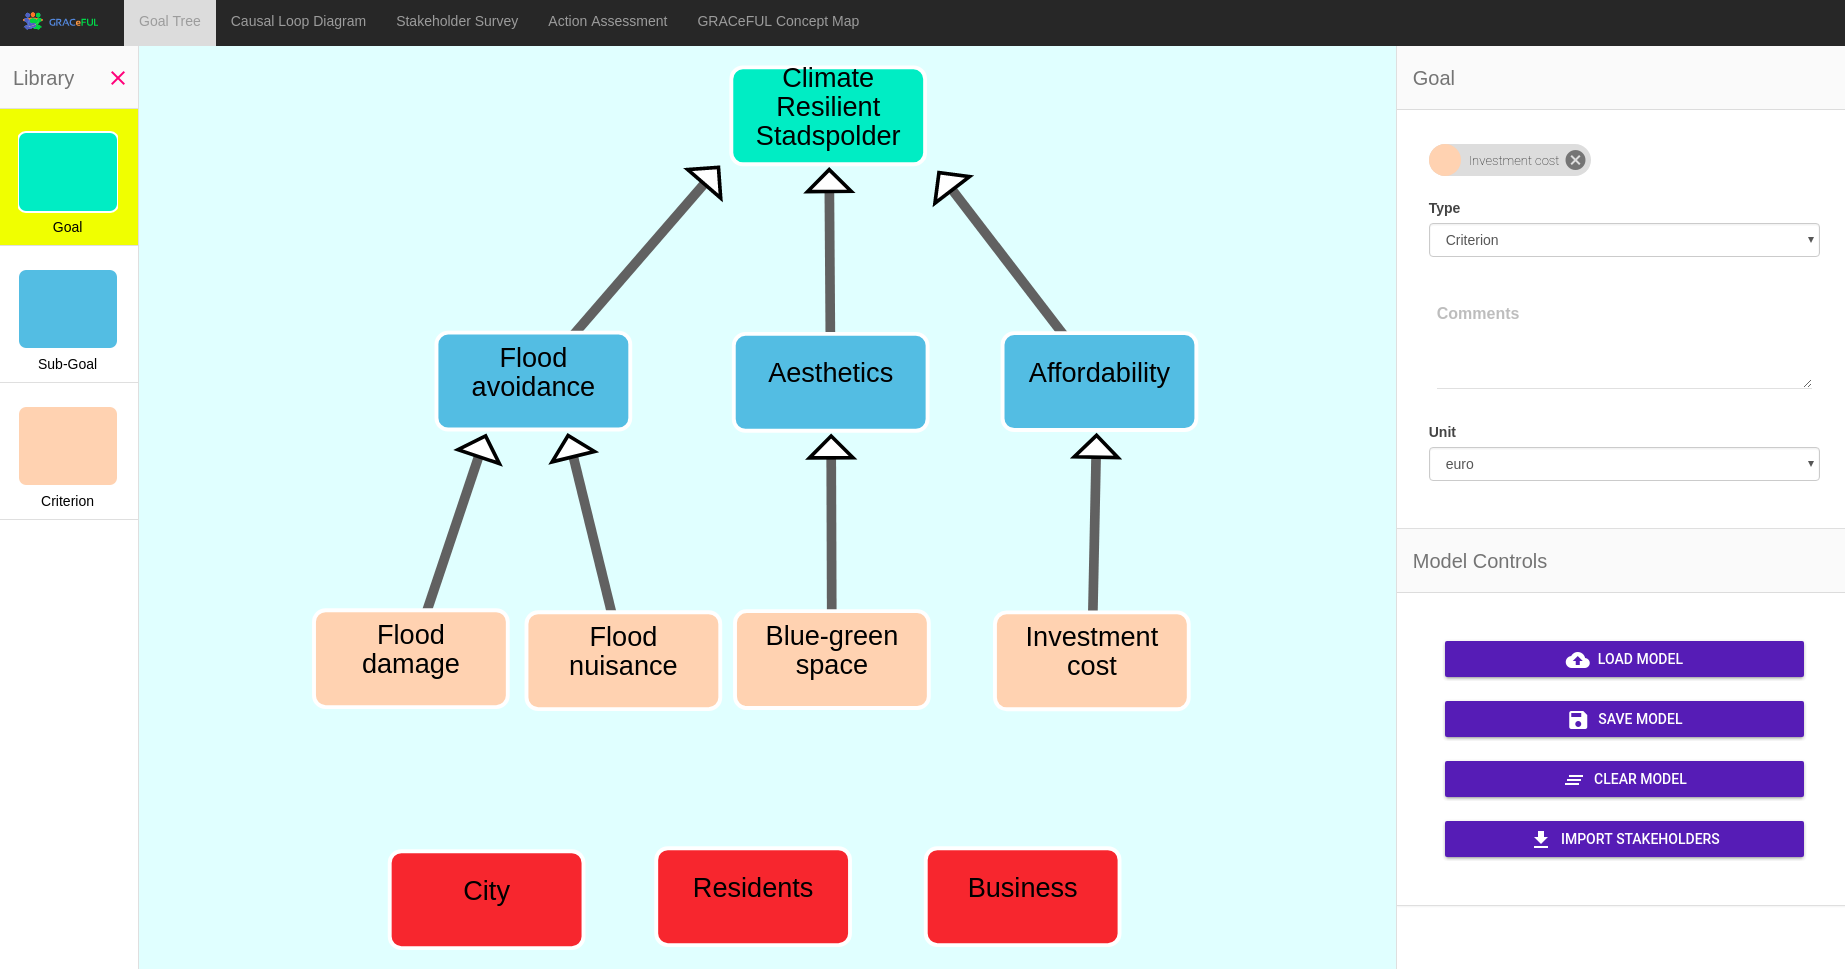
\includegraphics[height=3in,width=5in]{img/goal_tree.png}
\caption{\small \sl Goal Tree.\label{fig:goal_tree}}
\end{center}
\end{figure}

\subsection{Causal Loop Diagram}

Once the goal tree has been constructed, switch tab to the Causal Loop Diagram. The criteria and stakeholder nodes would automatically appear in the CLD editor (Figure \ref{fig:cld1}), as they are relevant to building the system model. The three causal elements, namely \textit{factor}, \textit{action}, and \textit{criterion} are available in the tool bar. The criterion is the same element as it is in goal tree. Creating a new criterion in the CLD editor would automatically appear in the goal tree editor. The controls tab on the right provides model controls, which assists in building the system model and server controls, which is used to communicate with the solver to get the library, sending the model and getting its results.

\begin{figure}[H]
\begin{center}
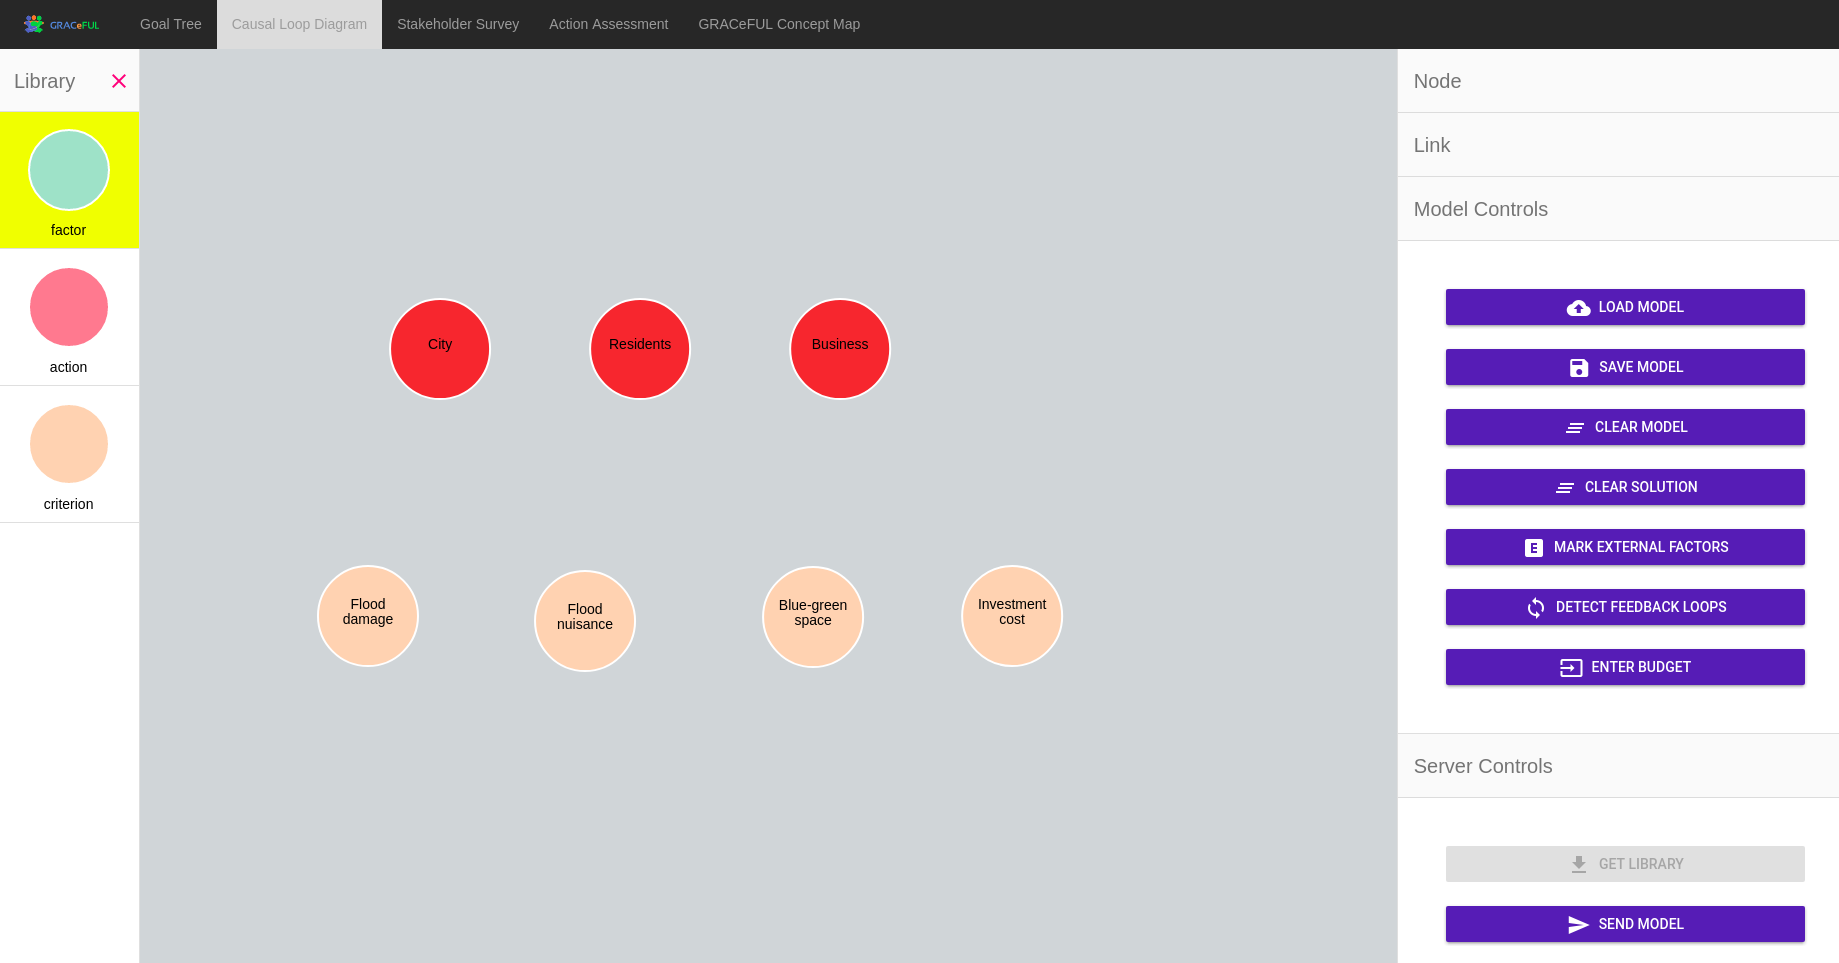
\includegraphics[height=3in,width=5in]{img/cld1.png}
\caption{\small \sl Initial view of Causal Loop Diagram.\label{fig:cld1}}
\end{center}
\end{figure}

\begin{figure}[H]
\begin{center}
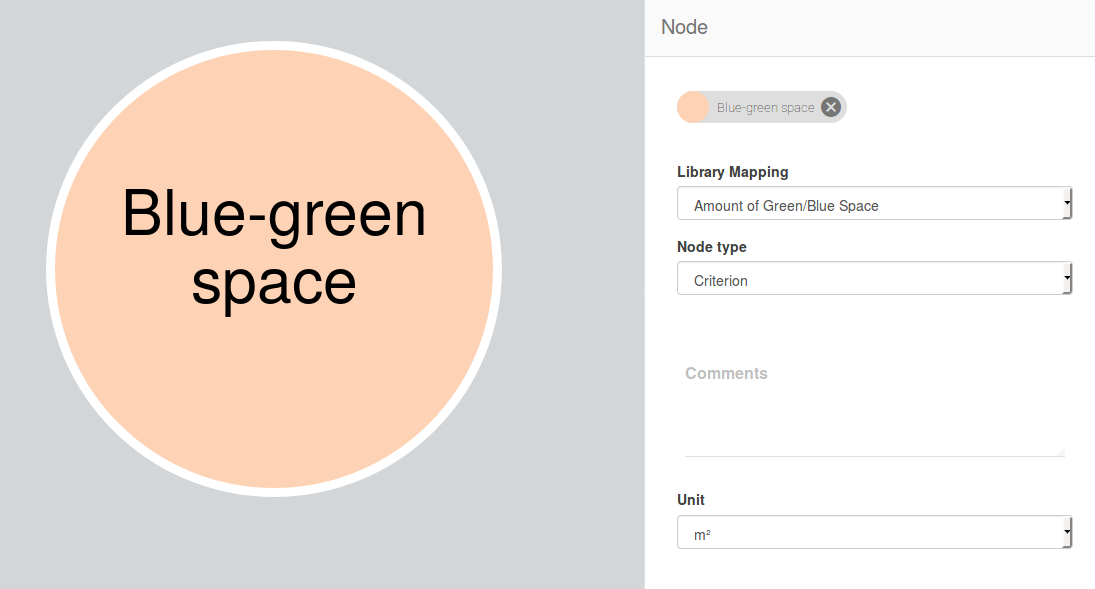
\includegraphics[width=0.75\linewidth, height=5cm]{img/criterion.png}
\caption{\small \sl A Criterion Node.\label{fig:criterion}}
\end{center}
\end{figure}

Figure \ref{fig:criterion} provides the attributes of a criterion node. During GMB, the stakeholders would suggest criteria and it is the responsibility of the modeler to map the criterion to the respective element in the library. In the future, this could be automatized through an intelligent linguistic mapping. The library mapping provides a list of standard criteria elements from the library for the modeler to choose the appropriate element for the criterion defined by the stakeholders.

The causal loop diagram is built by defining the factors and how they influence the identified criteria and other elements in the model. Figure \ref{fig:factors} shows the attributes of a factor node. In building a system model, it is possible to observe the trend of a factor to either increasing, decreasing, ambiguous, and stable. Selecting one of the option will result in a thick border around the node and the color indicates the selection type. Red indicates increasing, green indicates decreasing, gray with discontinuous border indicates ambiguous, and blue indicates stable. The factors that cannot be influenced by any other causal elements are identified as External Factors. They act as input to the system and are a source of uncertainty. The editor supports to find the external factors, by clicking on the \textit{Mark External Factors} button from the controls tab. They are colored dark gray for better visualization.

\begin{figure}[H]
\begin{subfigure}{1.0\textwidth}
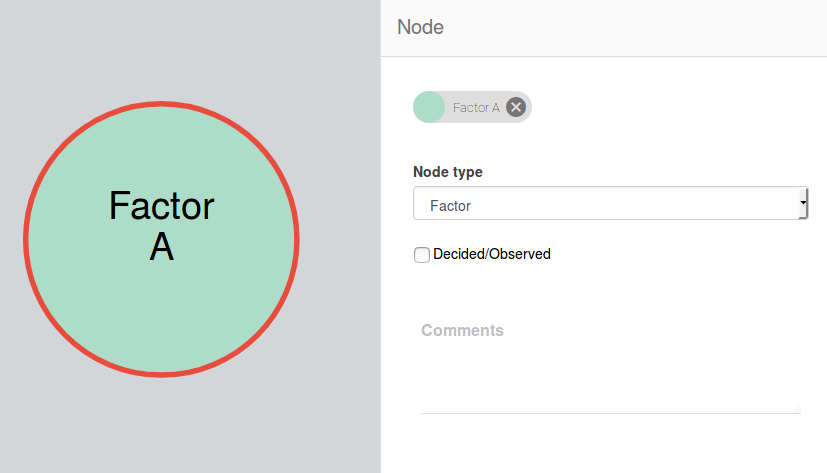
\includegraphics[width=0.75\linewidth, height=6cm]{img/factor.png} 
\caption{Without observe}
\label{fig:factor}
\end{subfigure}
\begin{subfigure}{1.0\textwidth}
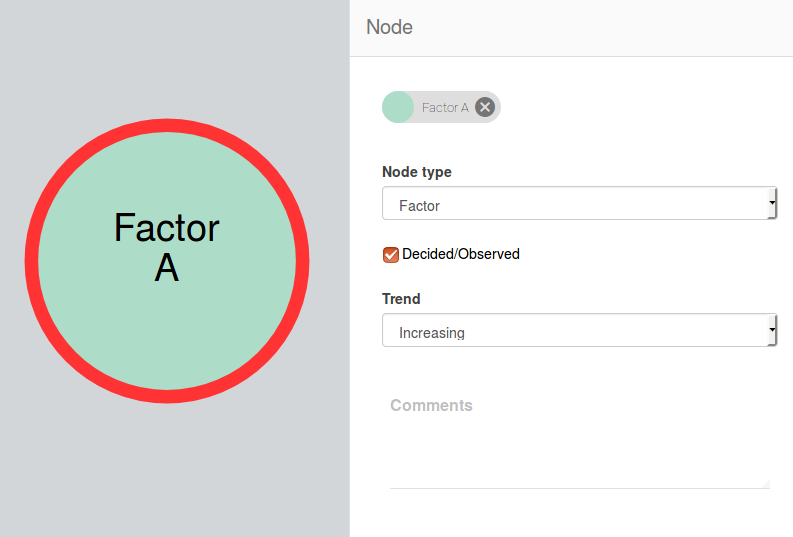
\includegraphics[width=0.75\linewidth, height=6cm]{img/factor1.png}
\caption{On observe}
\label{fig:factor1}
\end{subfigure}
\caption{A Factor Node.}
\label{fig:factors}
\end{figure}

In CLD, the factors and/or criteria are linked by causal relation links. The causal relation is represented by a directed link, annotated with a sign, which is plus or minus or question mark or zero. The sign plus signifies increasing causal relation, minus sign signifies decreasing causal relation, question mark sign signifies unknown/ambiguous causal relation, and zero sign signifies nothing, which is equivalent to being no link drawn at all. By default, the links have a causal relation sign plus annotated. Figure \ref{fig:links} shows the attributes of a causal relation link.

\begin{figure}[H]
\begin{center}
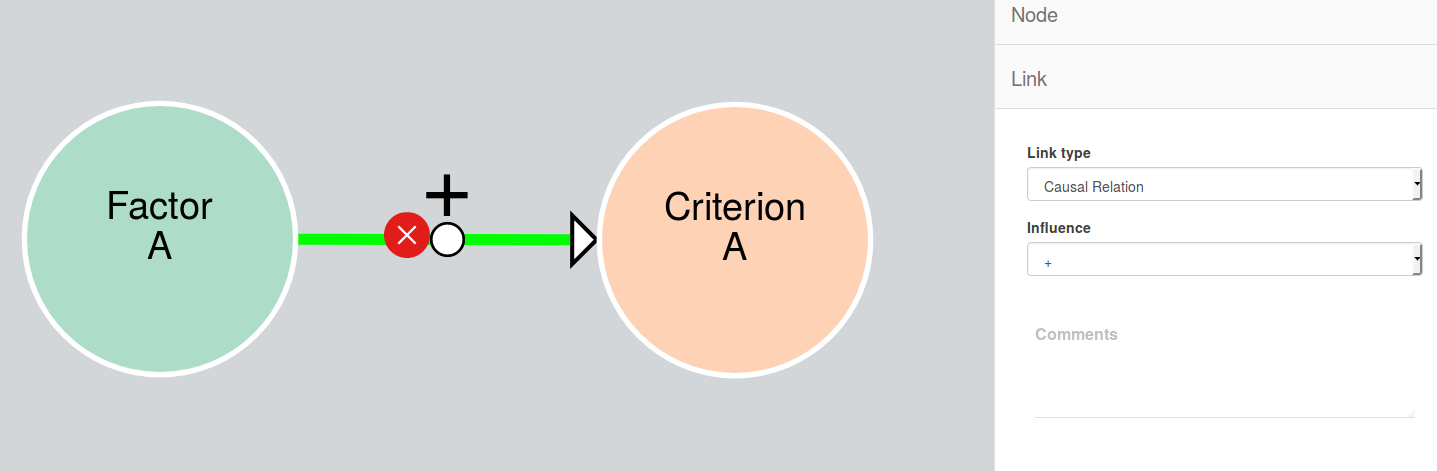
\includegraphics[width=1.0\linewidth, height=5cm]{img/links.png}
\caption{\small \sl Causal Relation.\label{fig:links}}
\end{center}
\end{figure}

\begin{figure}[H]
\begin{center}

\includegraphics[width=0.75\linewidth, height=6cm]{img/action.png}
\caption{\small \sl An Action Node.\label{fig:action}}
\end{center}
\end{figure}

The causal element Action helps the stakeholders to generate possible actions that can influence the criteria directly or through factors, based on the analysis of the system model. Again, the modeler has to map the action to the respective element in the library. The library mapping provides a list of standard action elements from the library for the modeler to choose the appropriate element for the action defined by the stakeholders. The attribute Action pairs indicates the cost associated in applying the action either positively (+), and/or negatively (-), and/or stable (0). An overall budget has to be defined first before applying the actions. To enter a budget in the editor, click on the button \textit{Enter Budget} from the controls tab and enter the maximum budget value as shown in the Figure \ref{fig:budget}. This is important as the solver would consider the maximum budget for applying the actions defined by the stakeholders.

\begin{figure}[H]
\begin{center}

\includegraphics[width=0.75\linewidth, height=4cm]{img/budget.png}
\caption{\small \sl Maximum Budget for the model.\label{fig:budget}}
\end{center}
\end{figure}

Once a CLD is built, it has to be checked for the presence of loops in the model. It is important to avoid them, otherwise the model would be inconsistent. The \textit{Detect Feedback Loops} button from the controls tab helps in identifying the loops. If the causal relation links in the loop contain an even number of minus sign, then the loop is referred to as reinforcement loop, otherwise the loop is referred to as balancing loop. Figure \ref{fig:loops} shows a simple graph with two loops. Right click on the link to add the feedback symbol. The editor would identify whether the symbol is either a reinforcement loop (R) or balancing loop (B) depending upon the number of minus sign causal relations.

\begin{figure}[H]
\begin{center}
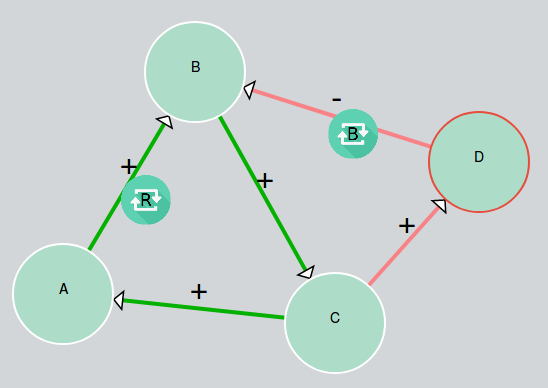
\includegraphics[width=0.75\linewidth, height=5cm]{img/loops.png}
\caption{\small \sl Feedback loops in the model.\label{fig:loops}}
\end{center}
\end{figure}

Figure \ref{fig:cld} provides the complete view of a CLD which includes factors and their causal relation to the criteria, actions and their direct and/or indirect relation to the criteria.

\begin{figure}[H]
\begin{center}
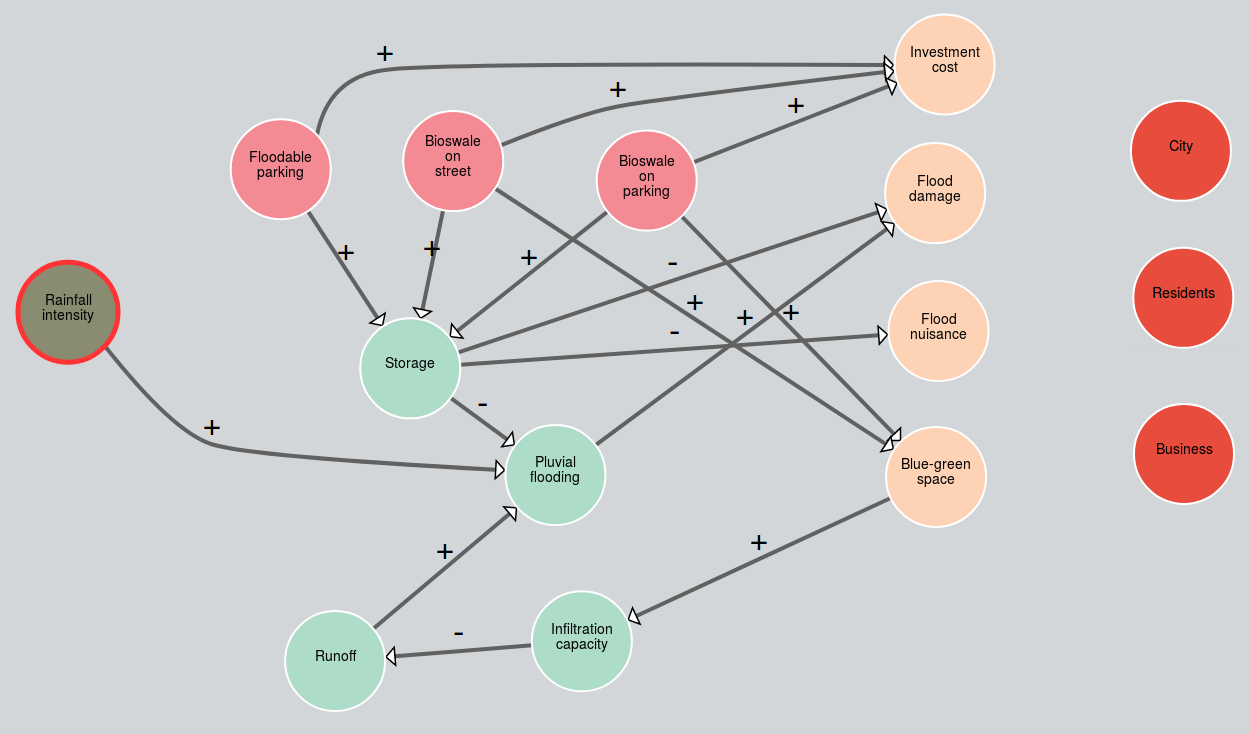
\includegraphics[height=3in,width=5in]{img/cld.png}
\caption{\small \sl Causal Loop Diagram with factors, actions, and causal relations.\label{fig:cld}}
\end{center}
\end{figure}

\subsection{Stakeholder Survey}

As mentioned earlier, the stakeholder participation in GMB is very important and hence it is necessary to collect their preferences for various criteria defined in the model. Switch tab to the Stakeholder survey in the editor and click on import model on the controls tab to load the table Stakeholder list along with the summary tables of stakeholder weights and values. Figure \ref{fig:sList} shows the stakeholder list table.

There are two ways to access the survey. The first option would be to click on the Create button in the table stakeholder list and save the file for every stakeholder. This file is sent to the stakeholder by email manually. The second option is to click on the MailTo button in the table stakeholder list and send the information by email. But, there are two problems associated with this. First, the mail client of the sender has to be configured in their system and second, the recipient has to store this information in a file manually before using it. Hence, it is advisable to use the first option.

\begin{figure}[H]
\begin{center}
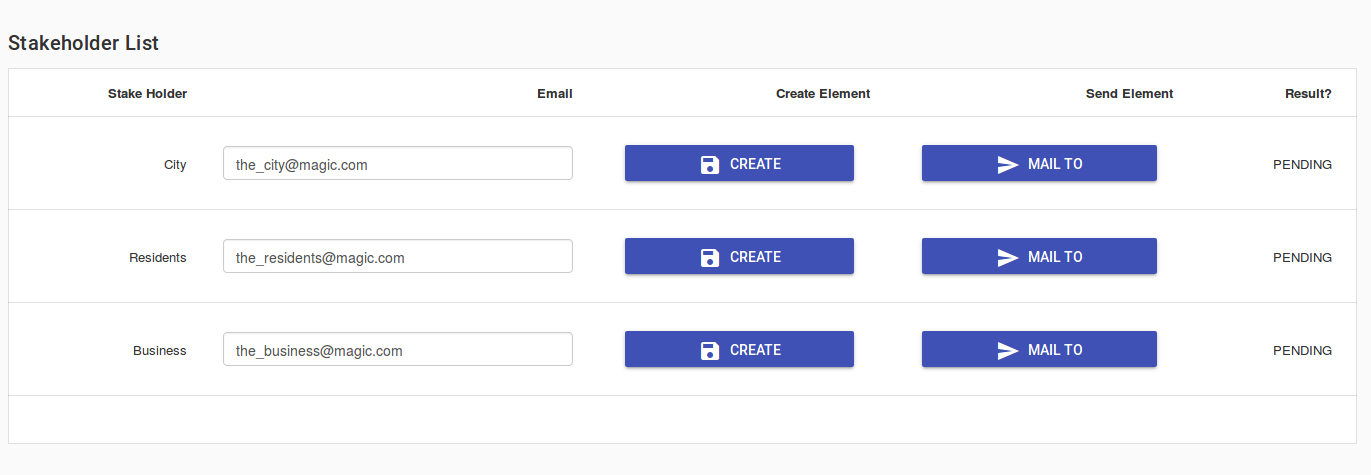
\includegraphics[height=2in,width=5in]{img/sList.png}
\caption{\small \sl Stakeholder Survey List.\label{fig:sList}}
\end{center}
\end{figure}

Once the stakeholder receives the file, the questionnaire page is opened using the url \url{http://vocol.iais.fraunhofer.de/graceful-rat/static/questioner.html}. Click on the button Load survey and select the respective file. Figure \ref{fig:weights} shows the table to weigh the criteria and follow the instructions to weigh them accordingly. Upon clicking the next button, Figure \ref{fig:values} shows the table to provide the constraints/values for every criteria. On complete, click on finish button and save the file. Send this saved file back to the facilitator by email manually.

\begin{figure}[H]
\begin{center}
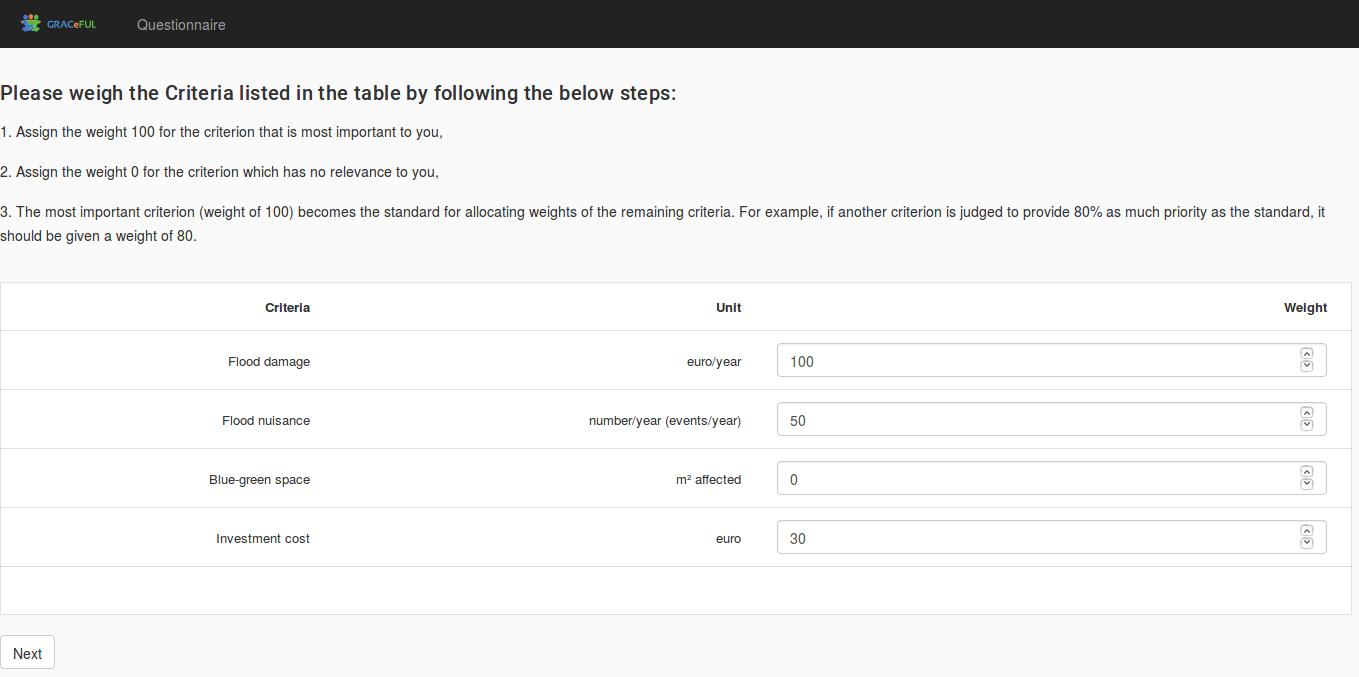
\includegraphics[width=6in, height=3in]{img/weights.png}
\caption{\small \sl Stakeholder providing weights.\label{fig:weights}}
\end{center}
\end{figure}

\begin{figure}[H]
\begin{center}
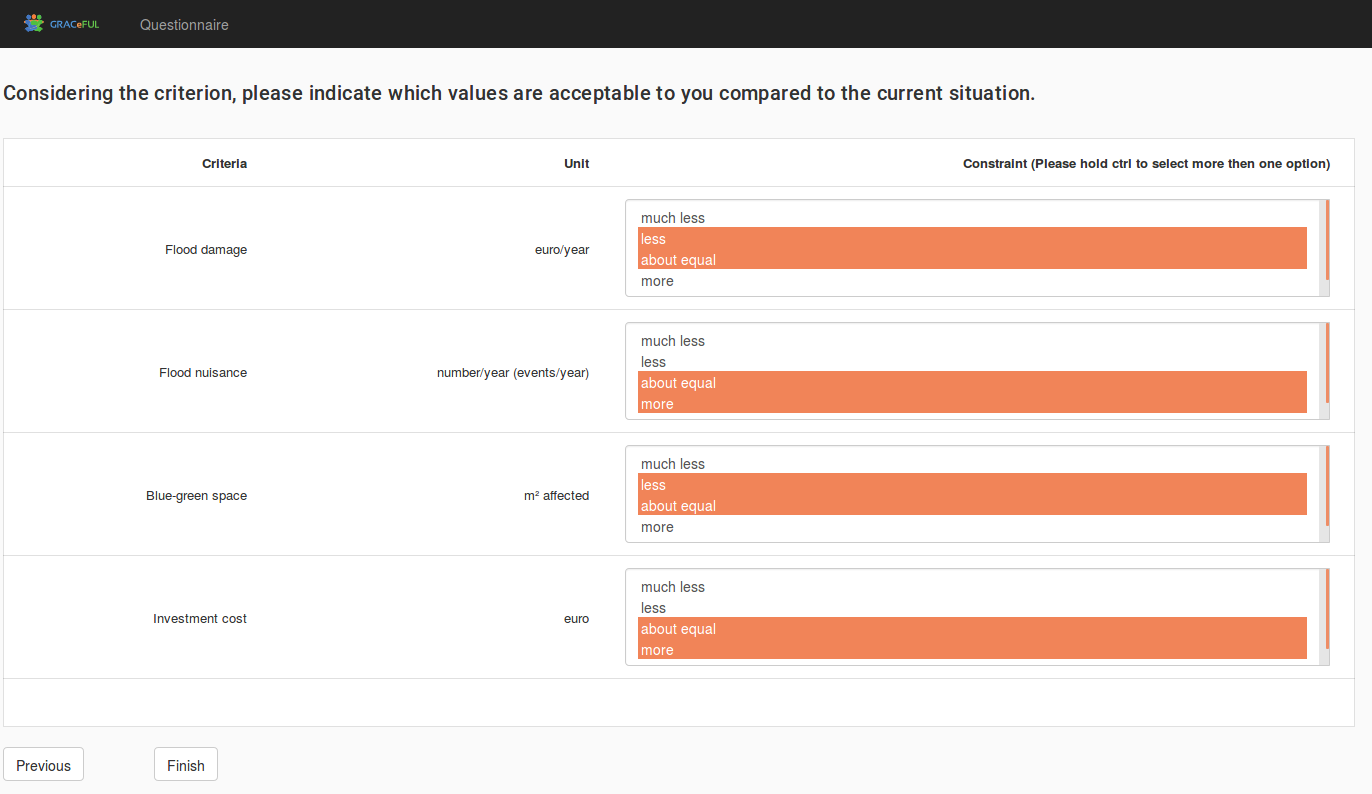
\includegraphics[width=6in, height=3in]{img/values.png}
\caption{\small \sl Stakeholder providing constraints/values.\label{fig:values}}
\end{center}
\end{figure}

Once the facilitator receives all the survey result files, click on the Load results button in the Stakeholder survey tab and select all the result files from the stakeholders and load them. The summary table shows the results of the stakeholder's weights and values as shown in the Figure \ref{fig:sSummary}. The stakeholder weights and values table is editable by the facilitator. If the weights and values has been edited, then the facilitator has to update it by clicking on the update button at the bottom.

\begin{figure}[p]
\begin{center}
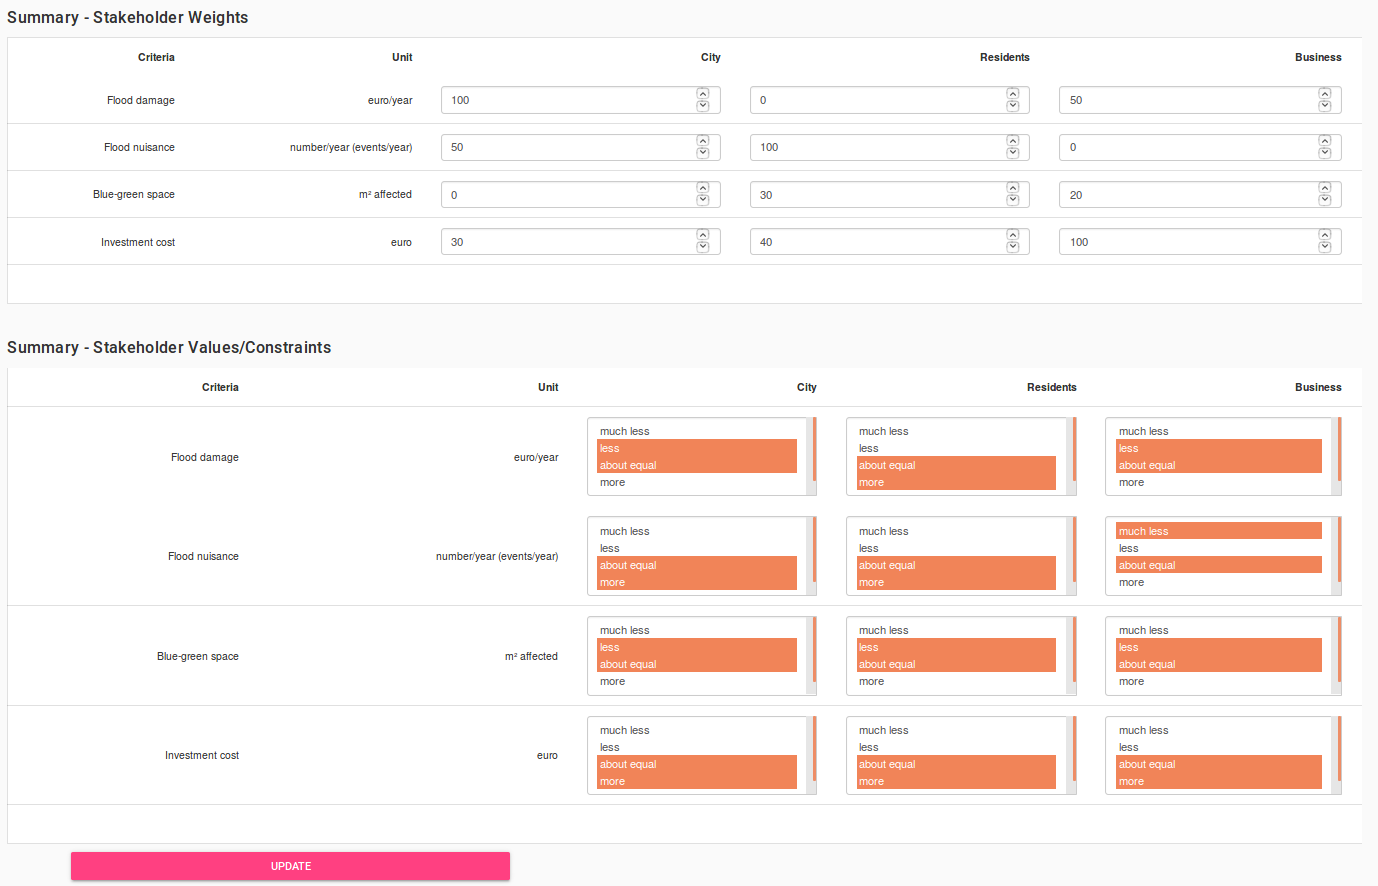
\includegraphics[width=6in, height=5in]{img/sSummary.png}
\caption{\small \sl Summary of Stakeholder Survey.\label{fig:sSummary}}
\end{center}
\end{figure}

The resultant of the stakeholder survey can be visualized in the CLD editor. Switch tabs to the CLD editor and a yellow link will be drawn between the stakeholder node and criteria, which they have weighed more than 0. On hovering over the stakeholder links, the normalized weight and its value can be viewed as shown in the Figure \ref{fig:cld2}. The normalized weight is the respective weight of a criterion divided by the sum of weights for all criteria assigned by a stakeholder and 0 represents about equal, 1 represents more, 2 represents much more, -1 represents less, and -2 represents much less. This completes the CLD model and it could be sent to the solver by clicking on the \textit{Send model} in the controls tab to get the results.

\begin{figure}[H]
\begin{center}
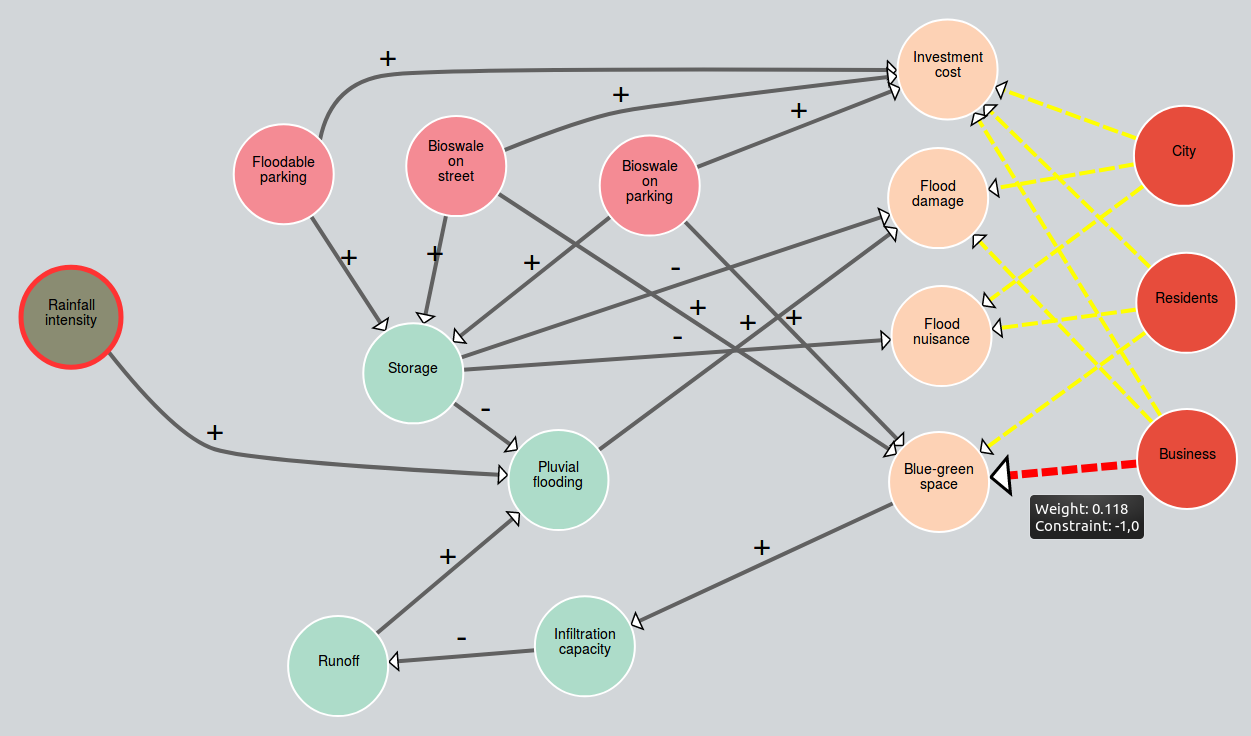
\includegraphics[height=3in,width=5in]{img/cld2.png}
\caption{\small \sl Causal Loop Diagram with Stakeholder links.\label{fig:cld2}}
\end{center}
\end{figure}

Figure \ref{fig:result} shows the result obtained from the solver for the CLD model. For every causal node, a color dot signifies its result. Red indicates its result is increasing, green indicates its result is decreasing, gray indicates its result is unknown/ambiguous, and blue indicates stable. The happiness of every stakeholder is found out by clicking on the stakeholder node and finding the happiness in the controls tab, which is expressed in a decimal form between 0 to 1. If required, the result can be cleared by clicking on the clear solution button in the controls tab.

\begin{figure}[H]
\begin{center}
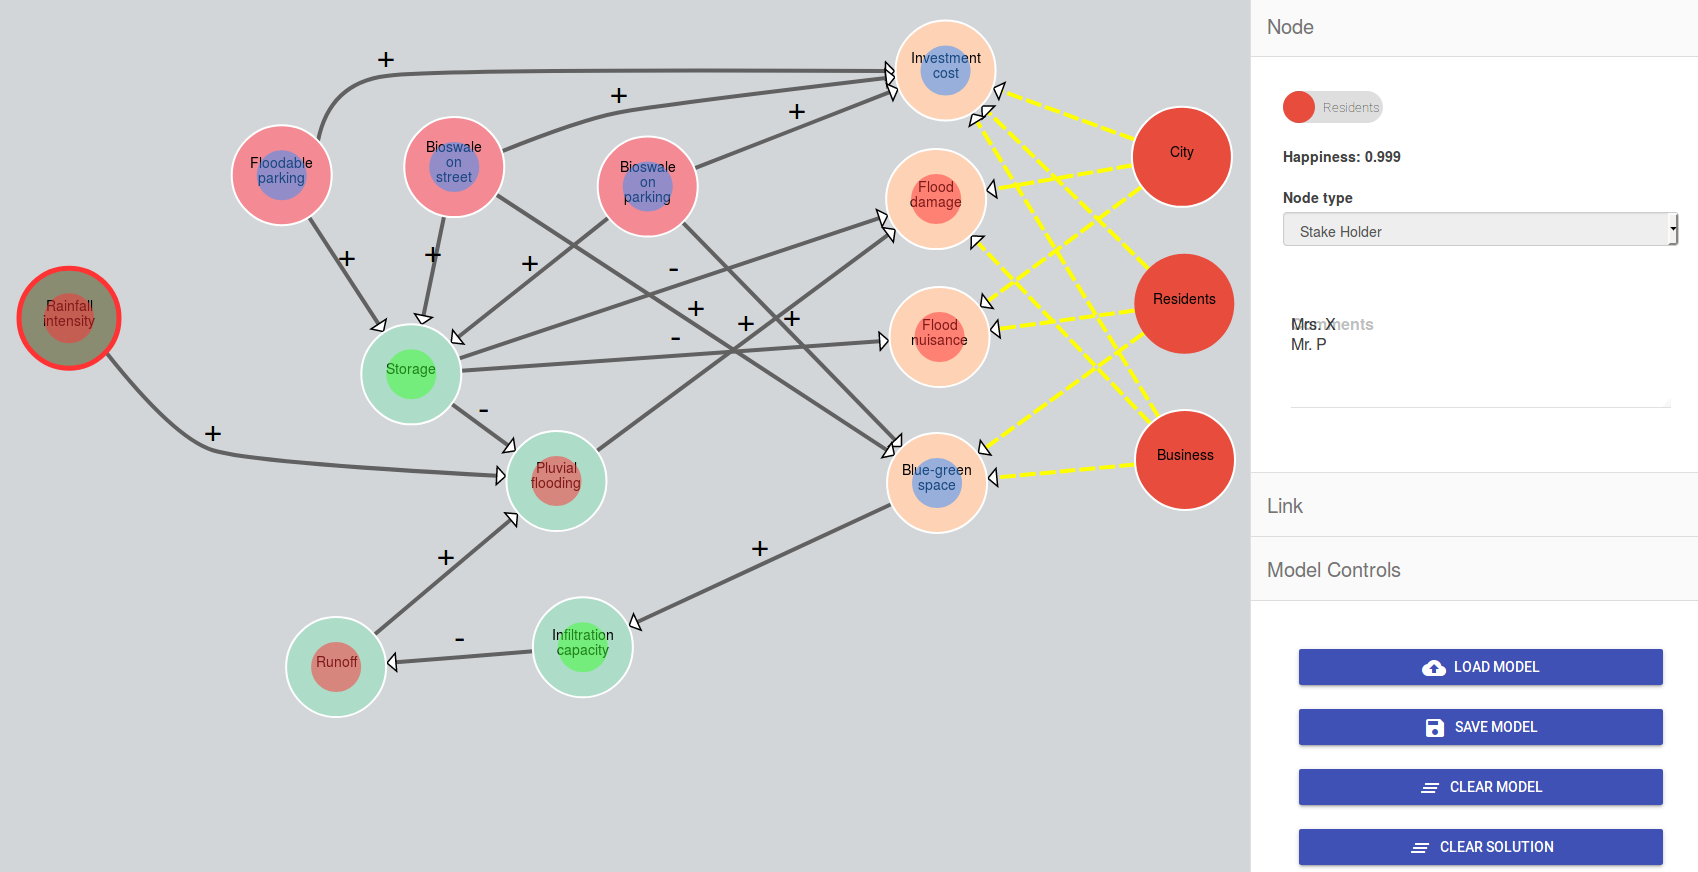
\includegraphics[height=3in,width=5in]{img/result.png}
\caption{\small \sl Result of the Causal Loop Diagram Model.\label{fig:result}}
\end{center}
\end{figure}

\begin{figure}[H]
\begin{center}
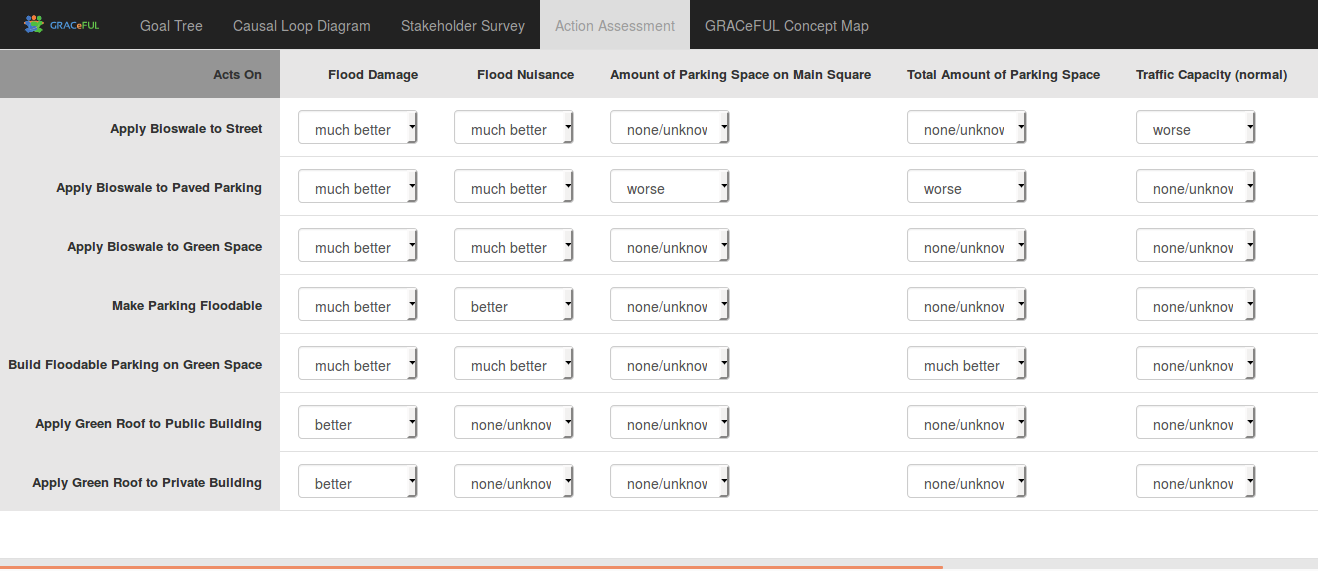
\includegraphics[width=6in, height=3in]{img/assess.png}
\caption{\small \sl Action Assessment.\label{fig:assess}}
\end{center}
\end{figure}

\begin{figure}[H]
\begin{center}
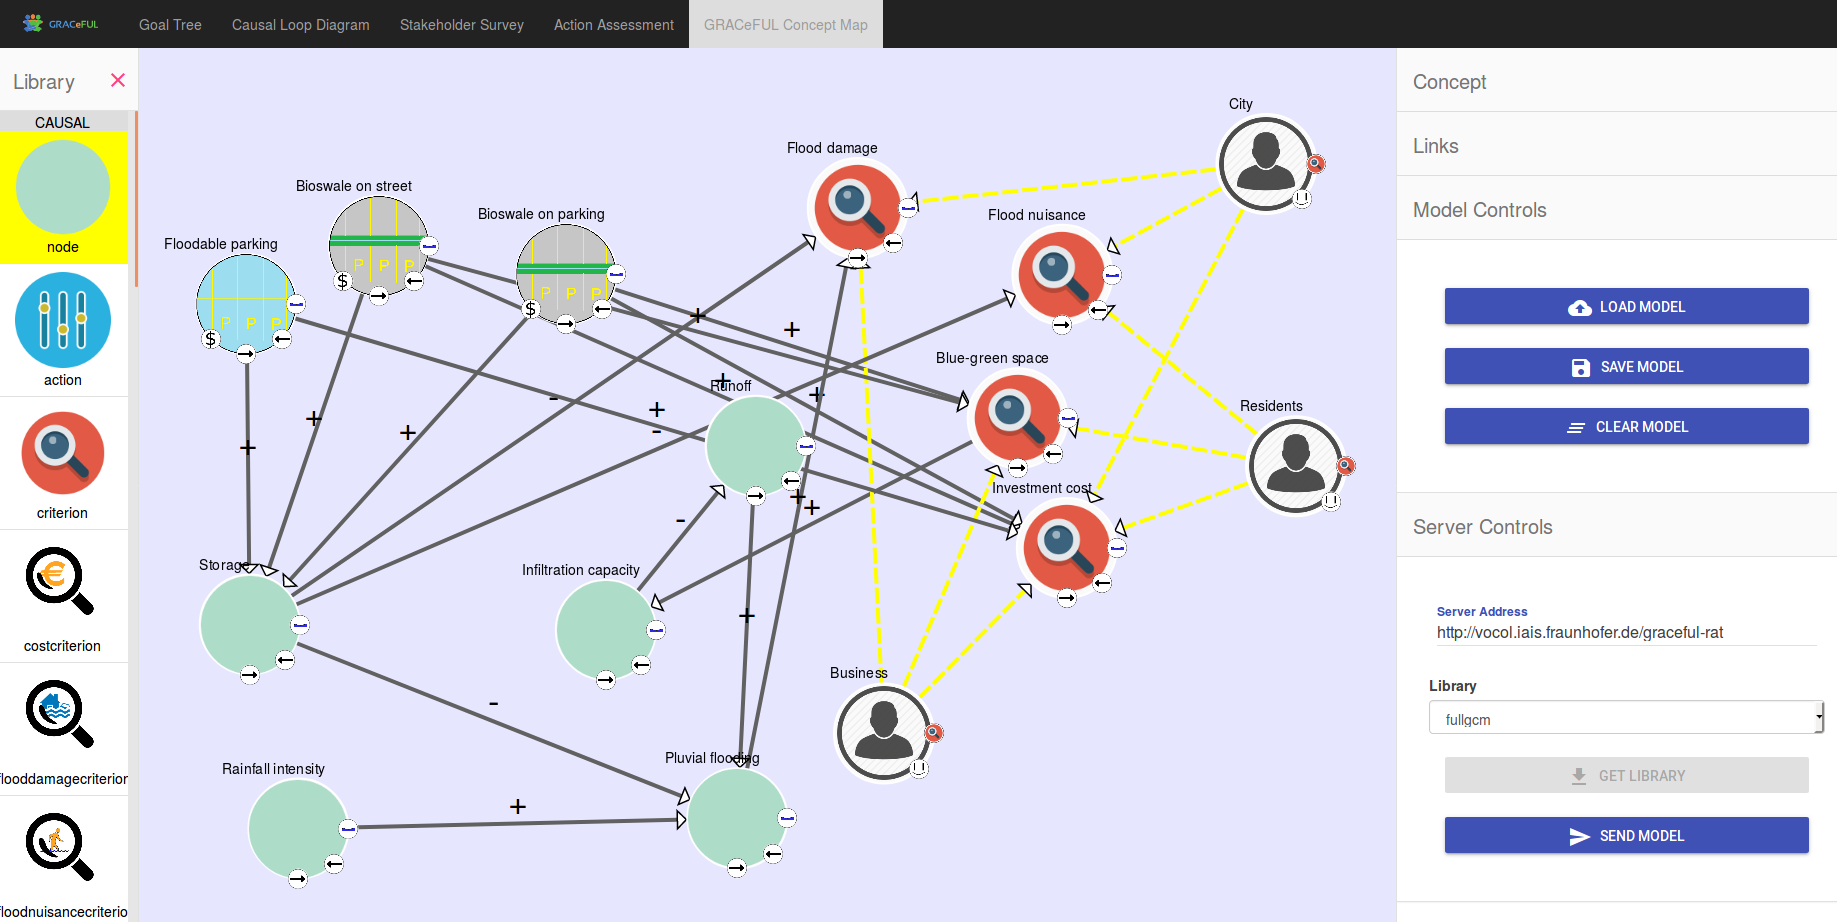
\includegraphics[height=3in,width=5in]{img/gcm.png}
\caption{\small \sl Graceful Concept Map.\label{fig:gcm}}
\end{center}
\end{figure}

\subsection{Action Assessment}

The action assessment tab contains the table (Figure \ref{fig:assess}) with Actions as rows and Criteria as columns and its respective value is set by the solver. It has one of the possible five values: much better, better, none/unknown, worse, and much worse. This table would assist the facilitator in filtering the actions out of all possible actions obtained from the solver in the Graceful Concept Map.

\subsection{Graceful Concept Map}

The Graceful Concept map is also synced with the goal tree and causal loop diagram and the model created in CLD would appear automatically as shown in the Figure \ref{fig:gcm}. Addtionally, more elements from the library can be used to add quantitative information to the model. The toolbar consists of all the library elements obtained from the engine.

\newpage

\section{Design and Implementation}
\label{implementation}

In this section, we provide the technical design and working of the visual editor. As introduced, it is a web-based application, which is implemented using HTML, CSS and JavaScript.  

Figure \ref{fig:visual} provides the different components of the visual editor. HTML helps in describing the structure of the application and CSS helps in better presentation of the HTML elements with proper layouts, colors, fonts, etc. JavaScript is an untyped scripting language, which helps in initializing and accessing the HTML Document Object Model (DOM) elements and also to dynamically load and change the visual appearance of the DOM. The communication module is responsible for communicating with the engine to fetch the library components and to send the model for evaluation. To have a better visual appearance, the editor uses Bootstrap, which is a HTML, CSS, and JavaScript framework. It helps in responsive design of the application, which allows it to adapt to different screen sizes, such as mobiles, tablets, desktops.

\begin{figure}
\begin{center}
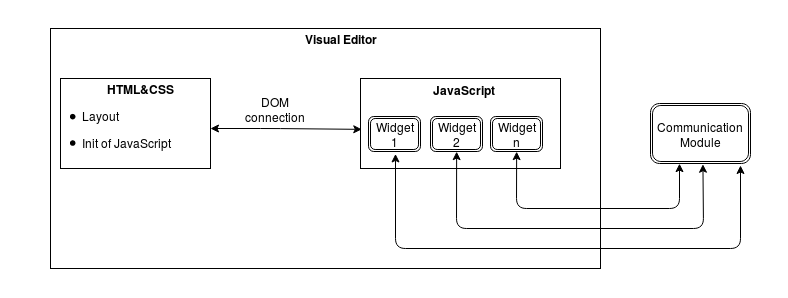
\includegraphics[height=2in,width=5in]{img/visual.png}
\caption{\small \sl Visual Editor Components.\label{fig:visual}}
\end{center}
\end{figure}

The visual editor follows a Widget-based design. The general idea is to use widgets to encapsulate different steps in the model building process. That is, the Goal Tree, CLD, SFD-like diagrams, which are available as separate tabs in the editor are individual widgets that provides its own Graph, Options/Controls, CSS styles, and type as illustrated in Figure \ref{fig:widget}.

\begin{figure}
\begin{center}
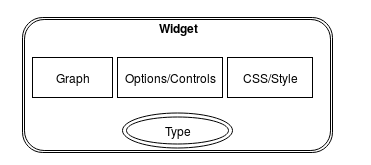
\includegraphics[height=2in,width=4in]{img/widget.png}
\caption{\small \sl Composition of a Widget.\label{fig:widget}}
\end{center}
\end{figure}

The graph is the main canvas area, which provides the rendering for nodes and links. All nodes and links are Scalable Vector Graphic (SVG) elements. We use D3.js, which is a JavaScript library for dynamic visual interaction. The options/control component contains the control buttons to edit, delete nodes and links and connect to the communication module. The CSS styles are responsible for manipulating the styles of the corresponding widget. The type signifies the widget’s type, i.e., goal tree, CLD, SFD-like diagrams, which is important for the communication module.

The widgets are rendered in the browser as separate tabs in the navigation bar that allows switching between different views of the editor. A new view can be easily created by extending the base widget and customizing it to our requirements.

\begin{figure}
\begin{center}
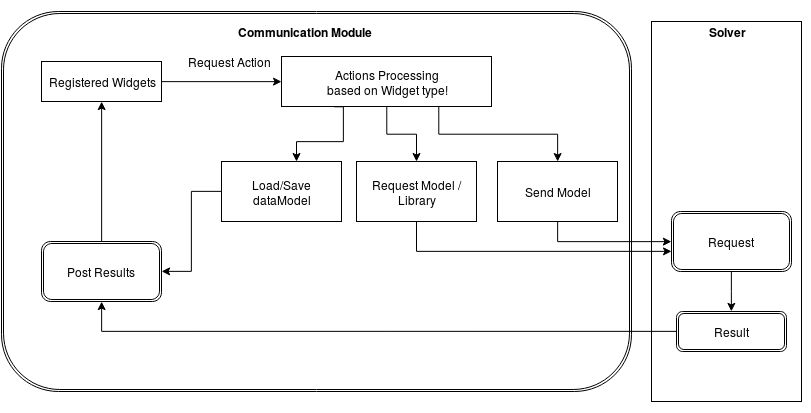
\includegraphics[height=3in,width=5in]{img/communication.png}
\caption{\small \sl Working of the Communication module.\label{fig:communication}}
\end{center}
\end{figure}

Figure \ref{fig:communication} provides the working details of the communication module. All widgets register to this module. The control component in the widget requests for action, such as load/save previous state, request library, send a model. An action is preprocessed based on the type of the widget. When sending the model, only the required data is sent to the engine. The request is either sent to the engine or, in case of loading a previous state, it directly goes to the Post results, which communicates the new results to the widget that requested this action. The widget then only needs to update itself. The communication module encapsulates the communication between the visual editor and the engine. It will be easier to maintain and modify the whole back-end communication with this module, but it requires an implementation for each widget.

Currently, the visual editor is deployed in a container to ease the process of testing while communicating to the engine. This Docker image is being deployed on a server.

\begin{figure}
\begin{center}
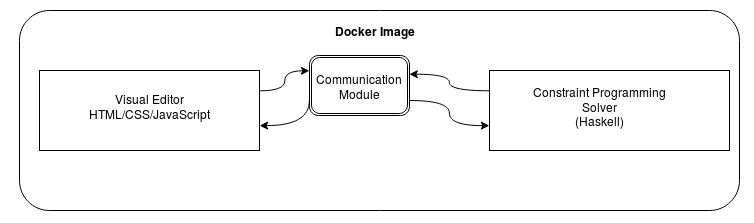
\includegraphics[height=1.5in,width=4in]{img/e2e.png}
\caption{\small \sl Docker image of the visual editor.\label{fig:e2e}}
\end{center}
\end{figure}


\end{document}